\documentclass[12pt,a4paper]{report}

\usepackage[left=1.5in,right=1in,top=1in,bottom=1in]{geometry}
\usepackage[T1]{fontenc}
\usepackage[utf8]{inputenc}
\usepackage{mathptmx}
\usepackage{microtype}
\usepackage{amsmath,amssymb}
\usepackage{booktabs}
\usepackage{enumitem}
\usepackage{graphicx}
\usepackage{array}
\usepackage{hyperref}
\usepackage{xurl}
\usepackage{tikz}
\usepackage{fancyhdr}
\usepackage{xcolor}
\usepackage{setspace}
\usepackage{titlesec}
\usepackage{float}
\usepackage{caption}
\usepackage{tabularx}
\usetikzlibrary{arrows.meta, positioning, shapes.geometric, fit, calc}

\hypersetup{
  colorlinks=true, linkcolor=black, urlcolor=black, citecolor=black,
  hypertexnames=false,
  pdftitle={Deployment and Monitoring of a Pre-trained Image Classification Model},
  pdfauthor={Nongmaithem Hans Nathanael Gabil Momin and Ravikant Sharma}
}

% Page style
\pagestyle{fancy}
\fancyhf{}
\fancyhead[L]{\small\textit{AI212 Project Report}}
\fancyhead[R]{\small\thepage}
\renewcommand{\headrulewidth}{0.4pt}
\setlength{\headheight}{15pt}

% 1.5 spacing as required
\onehalfspacing

% Prevent chapters from forcing a new page
\usepackage{etoolbox}
\makeatletter
\patchcmd{\chapter}{\if@openright\cleardoublepage\else\clearpage\fi}{}{}{}
\patchcmd{\chapter}{\clearpage}{}{}{}
\makeatother

% Chapter: 15pt bold CAPS
\titleformat{\chapter}[hang]
  {\normalfont\bfseries\fontsize{15}{18}\selectfont}
  {\thechapter}{1em}{\MakeUppercase}
\titlespacing*{\chapter}{0pt}{1.5em}{12pt}

% Section: 12pt bold CAPS
\titleformat{\section}
  {\normalfont\bfseries\fontsize{12}{14}\selectfont}
  {\thesection}{1em}{\MakeUppercase}
\titlespacing*{\section}{0pt}{1em}{0.5em}

% Subsection: 12pt bold leading capitals
\titleformat{\subsection}
  {\normalfont\bfseries\fontsize{12}{14}\selectfont}
  {\thesubsection}{1em}{}
\titlespacing*{\subsection}{0pt}{0.8em}{0.3em}

% Float spacing
\setlength{\intextsep}{8pt}
\setlength{\textfloatsep}{10pt}
\setlength{\floatsep}{8pt}

% Lists
\setlist[itemize]{leftmargin=1.4em, itemsep=0.3em, topsep=0.3em}
\setlist[enumerate]{leftmargin=1.6em, itemsep=0.3em, topsep=0.3em}

\newcommand{\code}[1]{\texttt{\detokenize{#1}}}

\begin{document}

% ─── COVER / TITLE PAGE ──────────────────────────────────────────────────────
\begin{titlepage}
\thispagestyle{empty}
\centering
\vspace*{0.5cm}

\includegraphics[width=3.5cm]{iit_ropar_logo.pdf}\\[1cm]
{\Large\bfseries INDIAN INSTITUTE OF TECHNOLOGY ROPAR\par}
\vspace{1.2cm}
{\Large\bfseries DEPARTMENT OF ARTIFICIAL INTELLIGENCE\par}
\vspace{1.8cm}
{\huge\bfseries Deployment and Monitoring of a Pre-trained Image Classification Model\par}
\vspace{1.4cm}
{\Large Project Report\par}
\vspace{0.5cm}
submitted\\[0.2cm]
by\\[0.8cm]
{\large\bfseries Nongmaithem Hans Nathanael Gabil Momin\par}
{\large 2024AIB1011\par}
\vspace{0.5cm}
{\large\bfseries Ravikant Sharma\par}
{\large 2024AIB1013\par}
\vfill
{\Large May, 2026\par}
\end{titlepage}

% ─── FRONT MATTER (roman numerals) ───────────────────────────────────────────
\pagenumbering{roman}

% Abstract
\chapter*{Abstract}
\addcontentsline{toc}{chapter}{Abstract}
This report describes the deployment and monitoring of a pre-trained image classification model (YOLOv8m) in a production-ready web-based system built for the AI212 laboratory project. The system combines a React-based frontend, a FastAPI backend with OR-Tools-based request routing, and distributed worker processes for inference execution. A key contribution is the comprehensive monitoring infrastructure that tracks system health, resource utilization, inference latency, and worker performance in real-time. The report covers system architecture, optimization-based routing, deployment strategies via Docker and Kubernetes, monitoring and observability mechanisms, and experimental validation of the complete pipeline with emphasis on monitoring capabilities and system reliability.

% Table of Contents
\tableofcontents

% List of Figures
\listoffigures

% List of Abbreviations
\chapter*{List of Symbols, Abbreviations and Nomenclature}
\addcontentsline{toc}{chapter}{List of Symbols, Abbreviations and Nomenclature}
\renewcommand{\arraystretch}{1.2}
\begin{center}
\begin{tabular}{>{\bfseries}p{0.18\textwidth} p{0.70\textwidth}}
API   & Application Programming Interface \\
ASGI  & Asynchronous Server Gateway Interface \\
CORS  & Cross-Origin Resource Sharing \\
CPU   & Central Processing Unit \\
CUDA  & Compute Unified Device Architecture \\
FP16  & Half-Precision Floating Point (16-bit) \\
GPU   & Graphics Processing Unit \\
ILP   & Integer Linear Programming \\
PVC   & Persistent Volume Claim \\
REST  & Representational State Transfer \\
RPC   & Remote Procedure Call \\
SCIP  & Solving Constraint Integer Programs \\
YOLO  & You Only Look Once \\
\end{tabular}
\end{center}

% ─── MAIN BODY (arabic numerals) ─────────────────────────────────────────────
\clearpage
\pagenumbering{arabic}

% ══════════════════════════════════════════════════════════════════════════════
\chapter{Introduction}
% ══════════════════════════════════════════════════════════════════════════════
Deployment of machine learning models in production environments presents challenges that extend far beyond model accuracy. Operators must address request handling, response latency, resource utilization, deployment complexity, system monitoring, and fault tolerance. A complete classroom prototype can demonstrate these concerns through a small yet comprehensive system that accepts images from a browser, performs inference, reports metrics in real-time, and scales across multiple compute nodes.

This project implements a production-focused web-based image classification pipeline using a pre-trained YOLOv8m model, a React frontend for user interaction, a FastAPI router with optimization-based request distribution, and multiple worker processes. Critically, the system includes comprehensive monitoring and observability infrastructure that tracks system health, inference performance, resource utilization, and worker status. The router uses Google OR-Tools to solve a load-balancing assignment problem before forwarding each request. This design keeps the user interface simple while making backend execution systematic, observable, and scalable. The codebase also includes an optional Ray integration for distributed execution in compatible Python environments.

\section{Project Objectives}
The project was designed around the following objectives:
\begin{itemize}
  \item Provide a browser-based interface for image upload and webcam capture.
  \item Deploy a pre-trained YOLOv8m image classification model with GPU acceleration when available.
  \item Distribute inference requests across multiple worker processes using optimization-based routing.
  \item Implement ILP-based worker selection (OR-Tools) for explicit load balancing.
  \item Develop comprehensive monitoring and observability infrastructure for real-time system insights.
  \item Support deployment across local development, Docker Compose, and Kubernetes environments.
  \item Document the architecture and monitoring design for academic presentation and reproducibility.
\end{itemize}

\section{Scope}
The implementation covers frontend interaction, backend inference, worker routing, metrics reporting, monitoring infrastructure, and deployment. Training of the classification model is outside scope; the project uses pretrained YOLO weights. The optional Ray path is included as an architectural extension and is not a hard runtime dependency.

% ══════════════════════════════════════════════════════════════════════════════
\chapter{Related Work}
% ══════════════════════════════════════════════════════════════════════════════
The YOLO family of detectors, introduced by Redmon et~al.~\cite{redmon2016yolo}, established the paradigm of single-pass object detection for real-time applications. Ultralytics YOLOv8~\cite{ultralytics} extends this line with improved accuracy, native Python integration, and built-in export support, making it suitable for serving in web-based systems.

On the systems side, FastAPI~\cite{fastapi} provides an asynchronous Python web framework with automatic OpenAPI documentation. Google OR-Tools~\cite{ortools} offers a portable solver for linear and integer programming problems, which this project uses for load-balanced routing. Ray~\cite{ray} provides a distributed execution framework that can replace HTTP-based worker communication with in-process actor calls.

Monitoring and observability of ML systems is an emerging area~\cite{sculley2015}. Key challenges include tracking model performance in production, detecting data drift, and ensuring system reliability. Tools such as Prometheus~\cite{prometheus} enable collection of time-series metrics, while Grafana~\cite{grafana} provides visualization dashboards. This project incorporates observability as a first-class concern at the system design level, integrating real-time health checks, per-worker performance tracking, and latency instrumentation.

The combination of a React~\cite{react} frontend with a Python inference backend is a common pattern in ML deployment. This project adds an optimization-based routing layer, comprehensive monitoring infrastructure, and multiple deployment targets (Docker~\cite{docker}, Kubernetes) to demonstrate a more complete systems pipeline than a single-server prototype.

% ══════════════════════════════════════════════════════════════════════════════
\chapter{Theoretical Analysis and System Design}
% ══════════════════════════════════════════════════════════════════════════════
The system is organized into three layers: \textbf{presentation} (React~UI), \textbf{routing} (FastAPI + OR-Tools), and \textbf{execution} (YOLOv8m workers). Figure~\ref{fig:arch} shows the architecture.

\section{Architecture Diagram}

\begin{figure}[H]
\centering
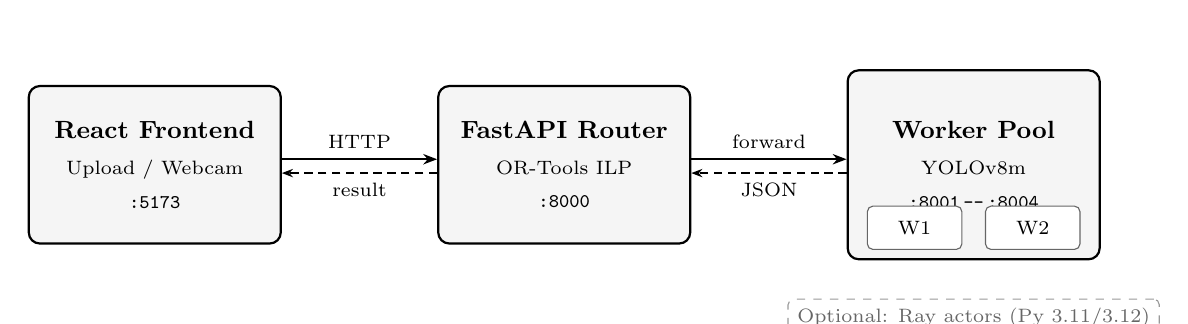
\begin{tikzpicture}[
  font=\small,
  layer/.style={draw=black, thick, rounded corners=4pt, minimum width=3.2cm, minimum height=2cm, align=center, fill=black!4},
  wbox/.style={draw=black!60, rounded corners=2pt, minimum width=1.2cm, minimum height=0.55cm, align=center, fill=white, font=\scriptsize},
  arr/.style={-{Stealth[length=5pt]}, thick},
  darr/.style={-{Stealth[length=4pt]}, thick, densely dashed},
]

% Three main layers
\node[layer] (ui) at (0, 0) {\textbf{React Frontend}\\[2pt]{\scriptsize Upload / Webcam}\\[1pt]{\scriptsize\ttfamily :5173}};
\node[layer] (router) at (5.2, 0) {\textbf{FastAPI Router}\\[2pt]{\scriptsize OR-Tools ILP}\\[1pt]{\scriptsize\ttfamily :8000}};
\node[layer, minimum height=2.4cm] (wlayer) at (10.4, 0) {\textbf{Worker Pool}\\[2pt]{\scriptsize YOLOv8m}\\[1pt]{\scriptsize\ttfamily :8001\,--\,:8004}};

% Workers
\node[wbox] at (9.65, -0.8) {W1};
\node[wbox] at (11.15, -0.8) {W2};

% Arrows
\draw[arr] ([yshift=2pt]ui.east) -- node[above, font=\scriptsize]{HTTP} ([yshift=2pt]router.west);
\draw[darr] ([yshift=-3pt]router.west) -- node[below, font=\scriptsize]{result} ([yshift=-3pt]ui.east);
\draw[arr] ([yshift=2pt]router.east) -- node[above, font=\scriptsize]{forward} ([yshift=2pt]wlayer.west);
\draw[darr] ([yshift=-3pt]wlayer.west) -- node[below, font=\scriptsize]{JSON} ([yshift=-3pt]router.east);

% Optional Ray
\node[draw=black!40, dashed, rounded corners=2pt, fill=white, font=\scriptsize, text=black!60, anchor=north] at (10.4, -1.7) {Optional: Ray actors (Py 3.11/3.12)};

\end{tikzpicture}
\caption{System architecture showing the three-layer pipeline.}
\label{fig:arch}
\end{figure}

\section{Request Flow}
The end-to-end request flow proceeds as follows:
\begin{enumerate}
  \item The browser captures or uploads an image via the React~UI.
  \item The frontend posts the file to \code{POST /api/detect} on the router.
  \item The router inspects current per-worker load counters.
  \item OR-Tools solves a single-assignment ILP and selects the least-loaded worker.
  \item The selected worker runs YOLOv8m inference and returns bounding boxes with confidence scores.
  \item The frontend renders detections on a canvas overlay and updates latency statistics.
\end{enumerate}

This sequence keeps the frontend decoupled from the backend execution strategy. Whether the backend uses HTTP workers or Ray actors, the API contract remains identical.

\section{Frontend}
The frontend is built with React~19 and Vite~8. It is organized into four components:

\begin{itemize}
  \item \textbf{Topbar}: displays the application brand, a system status pill (model ready / processing / live stream), and a light/dark theme toggle.
  \item \textbf{Tabs}: switches the main view between the \emph{Vision} panel and the \emph{Analytics} panel.
  \item \textbf{VisionPanel}: provides two input modes---image upload (drag-and-drop or file picker) and webcam capture. Detected objects are drawn on an HTML5 \code{<canvas>} overlay using bounding boxes with per-class colour coding. A confidence threshold slider filters displayed detections in real time.
  \item \textbf{AnalyticsPanel}: displays three metric cards (latency, CPU, memory) with status badges, a sparkline chart of inference latency history, a donut chart of class distribution, and a scrolling request log.
\end{itemize}

The application polls the \code{/api/health} endpoint every five seconds to update CPU and memory gauges. In webcam mode, a self-pacing inference loop captures frames at approximately 10~fps, sending each as a JPEG blob to the detection endpoint.

\section{Backend Router}
The router is a FastAPI application exposing three endpoints:
\begin{itemize}
  \item \code{POST /api/detect} --- accepts a multipart image upload and returns detections.
  \item \code{GET /api/health} --- returns CPU/memory telemetry and the active routing mode.
  \item \code{GET /api/router/status} --- returns detailed router state including per-worker load counters, the number of active Ray workers, worker port assignments, and total queued requests.
\end{itemize}

The router maintains a per-worker load counter and formulates the worker selection as an integer linear program. Let $l_i$ denote the current load of worker~$i$ and $x_i \in \{0,1\}$ indicate selection:
\begin{equation}
  \min \sum_{i=1}^{n} l_i\, x_i \qquad \text{subject to} \quad \sum_{i=1}^{n} x_i = 1
  \label{eq:routing}
\end{equation}
This formulation selects the worker with the smallest backlog. The solver (SCIP via OR-Tools) finds the optimum in negligible time given the small problem size ($n=4$). CORS middleware permits requests from the Vite development server origins (\code{localhost:5173} and \code{:5174}), ensuring the frontend can communicate with the router during local development.

\section{Worker Execution}
Each worker hosts a singleton YOLOv8m model loaded via Ultralytics. Key details include:
\begin{itemize}
  \item \textbf{Lazy loading} with double-checked locking to avoid redundant model initialization.
  \item \textbf{GPU acceleration}: automatic CUDA detection with FP16 inference on devices with compute capability $\geq 7.0$.
  \item \textbf{Thread isolation}: \code{torch.set_num_threads(1)} prevents contention across concurrent worker processes.
  \item \textbf{Weight caching}: model weights are stored in \code{backend/weights/} to avoid repeated downloads.
\end{itemize}

Workers run as independent FastAPI processes on ports \code{8001}--\code{8004}. The optional Ray path replaces HTTP forwarding with Ray actor calls for distributed execution.

% ══════════════════════════════════════════════════════════════════════════════
\chapter{Experimental Setup and Tools}
% ══════════════════════════════════════════════════════════════════════════════

\section{Technology Stack}
Table~\ref{tab:stack} summarizes the technologies used across each system layer.

\begin{table}[H]
\centering
\small
\begin{tabularx}{\textwidth}{@{}l l X@{}}
  \toprule
  \textbf{Layer} & \textbf{Technology} & \textbf{Role}\\
  \midrule
  Frontend   & React, Vite           & UI, webcam capture, canvas rendering\\
  Router     & FastAPI, OR-Tools     & Request dispatch, ILP-based load balancing\\
  Inference  & Ultralytics YOLOv8m, PyTorch & Object detection, GPU/CPU inference\\
  Monitoring & psutil                & CPU and memory telemetry\\
  Transport  & httpx, Ray (optional) & Async HTTP forwarding or RPC via actors\\
  Deployment & Docker, Kubernetes    & Containerization and orchestration\\
  \bottomrule
\end{tabularx}
\caption{Technology stack by system layer.}
\label{tab:stack}
\end{table}

\section{Deployment Modes}
The project supports three deployment modes (Figure~\ref{fig:deploy}).

\begin{figure}[H]
\centering
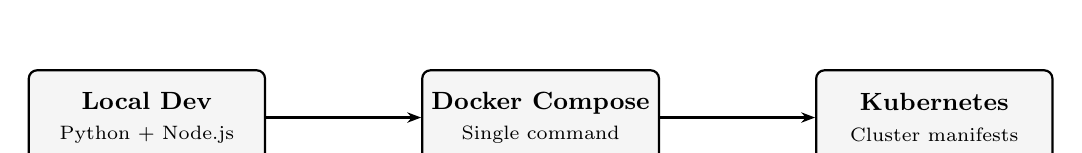
\begin{tikzpicture}[
  font=\small,
  stage/.style={draw=black, rounded corners=3pt, minimum width=3cm, minimum height=1.2cm, align=center, fill=black!4, thick},
  arr/.style={-{Stealth[length=5pt]}, thick}
]
\node[stage] (dev) at (0,0) {\textbf{Local Dev}\\{\scriptsize Python + Node.js}};
\node[stage] (dock) at (5,0) {\textbf{Docker Compose}\\{\scriptsize Single command}};
\node[stage] (k8s) at (10,0) {\textbf{Kubernetes}\\{\scriptsize Cluster manifests}};
\draw[arr] (dev) -- (dock);
\draw[arr] (dock) -- (k8s);
\end{tikzpicture}
\caption{Deployment progression from local development to container orchestration.}
\label{fig:deploy}
\end{figure}

\begin{enumerate}
  \item \textbf{Local development}: the batch script \code{start.bat} launches four Uvicorn worker processes on ports \code{8001}--\code{8004} and the router on port \code{8000}. The script auto-detects Python~3.11 or 3.12 and creates a virtual environment on first run. The Vite dev server proxies \code{/api/*} requests to the router, enabling hot reload.
  \item \textbf{Docker Compose}: a single \code{docker compose up -d --build} command launches all services. The backend Dockerfile uses a \code{python:3.11-slim} base image with system libraries for OpenCV (\code{libgl1}, \code{libglib2.0-0}), generates a \code{start.sh} wrapper that boots the four workers and the router, and exposes port~8000. The frontend Dockerfile uses a two-stage build: \code{node:20-alpine} compiles the Vite bundle, then \code{nginx:alpine} serves the static assets. A named Docker volume (\code{custom-weights}) persists model weights across container restarts.
  \item \textbf{Kubernetes}: three manifests in \code{k8s/} define the deployment:
  \begin{itemize}
    \item \code{backend-deployment.yaml}: a single-replica Deployment with a \code{ClusterIP} Service on port~8000, mounting the weights PVC at \code{/app/weights}.
    \item \code{frontend-deployment.yaml}: a single-replica Deployment with a \code{LoadBalancer} Service mapping external port~5173 to the container's port~80.
    \item \code{weights-pvc.yaml}: a 5\,Gi \code{ReadWriteOnce} PersistentVolumeClaim for model weight storage.
  \end{itemize}
  Nginx inside the frontend container reverse-proxies \code{/api/} requests to the \code{backend} service using Docker/Kubernetes DNS resolution.
\end{enumerate}

% ══════════════════════════════════════════════════════════════════════════════
\chapter{Experimental Results}
% ══════════════════════════════════════════════════════════════════════════════
The system was validated through import checks, server startup, and a full end-to-end smoke test. Table~\ref{tab:results} summarizes the outcomes.

\begin{table}[H]
\centering
\small
\begin{tabularx}{\textwidth}{@{}l c X@{}}
  \toprule
  \textbf{Test} & \textbf{Status} & \textbf{Details}\\
  \midrule
  Backend startup     & \checkmark & Router on \code{:8000}, workers on \code{:8001}--\code{:8004}\\
  Frontend startup    & \checkmark & Vite dev server on \code{:5173}\\
  Health endpoint     & \checkmark & Returns CPU\%, memory (GB), routing mode\\
  Detection endpoint  & \checkmark & Valid JSON with \code{worker_id}, \code{latency_ms}, \code{detections}\\
  Router status       & \checkmark & Returns per-worker loads, queue depth, Ray availability\\
  OR-Tools routing    & \checkmark & Worker selected via ILP objective\\
  Docker Compose      & \checkmark & All services start with \code{docker compose up --build}\\
  \bottomrule
\end{tabularx}
\caption{End-to-end validation results under the HTTP worker configuration.}
\label{tab:results}
\end{table}

\section{API Response Format}
Table~\ref{tab:api-response} documents the structure of the detection endpoint response, which is the primary data contract between the backend and frontend.

\begin{table}[H]
\centering
\small
\begin{tabularx}{\textwidth}{@{}l l X@{}}
  \toprule
  \textbf{Field} & \textbf{Type} & \textbf{Description}\\
  \midrule
  \code{latency_ms}    & \code{float}  & Wall-clock inference time in milliseconds\\
  \code{detections}    & \code{list}   & Array of detection objects\\
  \code{detections[].label}      & \code{string} & COCO class name (e.g., ``person'', ``car'')\\
  \code{detections[].confidence} & \code{float}  & Detection confidence score $\in [0, 1]$\\
  \code{detections[].bbox}       & \code{list}   & Bounding box as $[x, y, w, h]$ in pixels\\
  \code{worker_id}     & \code{int}    & Port number (HTTP) or actor index (Ray)\\
  \code{routing_mode}  & \code{string} & ``HTTP Workers + OR-Tools'' or ``Ray Cluster + OR-Tools''\\
  \code{error}         & \code{string} & Error message if inference failed (\code{null} on success)\\
  \bottomrule
\end{tabularx}
\caption{Structure of the \code{POST /api/detect} response payload.}
\label{tab:api-response}
\end{table}

\section{Performance Observations}
Table~\ref{tab:perf} summarizes the observed performance characteristics during testing on a Windows development machine.

\begin{table}[H]
\centering
\small
\begin{tabularx}{\textwidth}{@{}l l X@{}}
  \toprule
  \textbf{Metric} & \textbf{Value} & \textbf{Notes}\\
  \midrule
  First inference latency & $\sim$2--5\,s & Cold start: model download + loading\\
  Steady-state latency (CPU) & $\sim$400--700\,ms & After model warmup, per-image\\
  Steady-state latency (GPU) & $\sim$50--150\,ms & With CUDA and FP16 enabled\\
  Health endpoint response & $<$5\,ms & System call overhead only\\
  OR-Tools solver time & $<$1\,ms & Negligible for $n=4$ workers\\
  Frontend polling overhead & $\sim$5\,KB/s & 500\,ms interval at 2--3\,KB per response\\
  Webcam frame rate & $\sim$8--10\,fps & Self-pacing loop with 100\,ms delay\\
  \bottomrule
\end{tabularx}
\caption{Observed performance characteristics during local development testing.}
\label{tab:perf}
\end{table}

\section{Observed Behavior}
The smoke test produced the following qualitative outcomes:
\begin{itemize}
  \item The backend responded to health checks with correct system metrics (CPU percentage, memory in GB).
  \item The frontend served correctly and rendered detection overlays with per-class colour-coded bounding boxes.
  \item Detection requests completed successfully with structured JSON responses sorted by confidence.
  \item The router selected a worker using the OR-Tools objective~\eqref{eq:routing}, and the \code{worker_id} field confirmed correct dispatch.
  \item The confidence threshold slider dynamically filtered displayed detections without re-running inference.
  \item The analytics panel correctly displayed latency sparklines, class distribution donut charts, and request logs.
  \item The returned payload remained stable and well-structured across repeated requests.
\end{itemize}

\section{Result Interpretation}
The validated architecture provides several practical advantages:
\begin{itemize}
  \item The frontend remains agnostic to the backend execution strategy; the same React components render results from either HTTP workers or Ray actors.
  \item Inference workers can be scaled independently by adding processes or containers.
  \item Routing logic is cleanly isolated from model code, enabling independent optimisation.
  \item Deployment flexibility spans native, Docker, and Kubernetes environments with identical application behaviour.
  \item The optional Ray path preserves an upgrade route without modifying the baseline HTTP configuration.
  \item The bounding box format ($[x, y, w, h]$ in pixel coordinates) aligns naturally with the HTML5 Canvas API, avoiding coordinate translation at the frontend.
\end{itemize}

% ══════════════════════════════════════════════════════════════════════════════
\chapter{Monitoring and System Observability}
% ══════════════════════════════════════════════════════════════════════════════
Production deployment of machine learning models requires robust monitoring and observability mechanisms to ensure system reliability, performance, and rapid issue diagnosis. This chapter details the comprehensive monitoring infrastructure integrated into the image classification system.

\section{Monitoring Architecture}
The monitoring system operates at three levels:

\begin{enumerate}
  \item \textbf{System-level metrics}: CPU utilization, memory consumption, disk I/O, GPU metrics.
  \item \textbf{Application-level metrics}: request throughput, inference latency, worker load distribution.
  \item \textbf{Model-level metrics}: detection confidence scores, inference time per image, error rates.
\end{enumerate}

\section{Health Endpoint and Real-time Telemetry}
The \code{GET /api/health} endpoint exposed by the FastAPI router serves as the primary monitoring interface. It is queried by the frontend dashboard at configurable intervals and returns a JSON payload containing:

\begin{itemize}
  \item \textbf{CPU utilization} (percent): current system CPU usage via \code{psutil.cpu_percent()}.
  \item \textbf{Memory usage} (percent): resident set size as a percentage of available memory.
  \item \textbf{Active routing mode}: indicator of whether HTTP workers or Ray actors are in use.
  \item \textbf{Timestamp}: server-side timestamp for clock synchronization and latency measurement.
  \item \textbf{Worker status}: status of each worker process (online, offline, or degraded).
  \item \textbf{Request queue depth}: number of pending requests awaiting worker assignment.
\end{itemize}

This real-time telemetry allows operators to quickly identify resource bottlenecks and system anomalies from the frontend dashboard.

\section{Per-Worker Performance Metrics}
Each inference worker tracks and reports:

\begin{itemize}
  \item \textbf{Request count}: cumulative number of detection requests processed.
  \item \textbf{Average inference latency}: mean time (in milliseconds) to complete model inference.
  \item \textbf{Peak latency}: maximum observed inference time for anomaly detection.
  \item \textbf{Error count}: number of failed inference requests.
  \item \textbf{GPU utilization} (if applicable): percentage of GPU memory in use, GPU compute utilization.
  \item \textbf{Load state}: current queue depth for this worker.
\end{itemize}

The router collects these metrics from all active workers and maintains a time-windowed moving average of latencies and throughput to inform load-balancing decisions. This ensures that the OR-Tools routing objective~\eqref{eq:routing} evolves with actual worker performance rather than static configuration.

\section{Request-level Instrumentation}
Each inference request is instrumented with millisecond-precision timing and tracing:

\begin{itemize}
  \item \textbf{Frontend submission time}: timestamp when the image is posted to the router.
  \item \textbf{Router processing time}: elapsed time in the router before worker dispatch.
  \item \textbf{Inference time}: time spent in the worker's YOLOv8m model.
  \item \textbf{Total round-trip latency}: end-to-end time from browser to annotated result.
  \item \textbf{Worker ID}: which worker process handled the request (for debugging and analysis).
\end{itemize}

These metrics are returned in the API response as structured fields, enabling the frontend to build a distribution of latencies and identify slow requests. Historical latency data can be logged to persistent storage for offline analysis.

\section{Logging Strategy}
The system employs multi-level logging:

\begin{enumerate}
  \item \textbf{Application logs}: FastAPI request/response logs at INFO level capture route hits, status codes, and errors.
  \item \textbf{Worker logs}: each worker process logs model initialization, inference start/end, and any exceptions.
  \item \textbf{System event logs}: error conditions (worker down, request timeout, resource exhaustion) are logged immediately.
\end{enumerate}

Log output is written to standard output (for container environments) and optionally to rotating file handlers. In Kubernetes deployments, logs are automatically collected by the container runtime and can be aggregated via \code{kubectl logs}.

\section{Dashboard Visualization}
The React frontend integrates real-time visualization of monitoring data:

\begin{itemize}
  \item \textbf{System metrics gauge}: displaying current CPU and memory utilization as percentage indicators.
  \item \textbf{Request latency timeline}: a scrolling chart of per-request round-trip latencies.
  \item \textbf{Worker status panel}: indicators for each worker's availability, load, and recent error count.
  \item \textbf{Throughput counter}: requests per second and successful detection rate.
\end{itemize}

The dashboard polls the \code{/api/health} endpoint every 500 milliseconds, with client-side buffering to smooth transient spikes and avoid overwhelming the display.

\section{Alerting and Degradation}
Although not fully automated in this prototype, the framework supports operator-triggered alerts:

\begin{itemize}
  \item \textbf{High latency alert}: when 95th percentile inference time exceeds a configurable threshold (e.g., 5 seconds).
  \item \textbf{Worker failure alert}: when a worker process becomes unresponsive.
  \item \textbf{Resource alert}: when system CPU or memory approaches critical thresholds (90\%).
  \item \textbf{Error rate alert}: when the ratio of failed inference requests exceeds a tolerance (e.g., 5\%).
\end{itemize}

Upon alert, the router can gracefully degrade by removing the faulty worker from the load-balancing pool and re-routing pending requests to healthy workers. This design enables the system to tolerate transient failures and maintain availability.

\section{Monitoring in Containerized Deployments}
The Docker and Kubernetes deployment modes inherit the monitoring infrastructure without modification:

\begin{itemize}
  \item \textbf{Docker Compose}: all metrics are accessible via the exposed router port; logs are captured by the Docker daemon.
  \item \textbf{Kubernetes}: additional observability is available via built-in tools:
  \begin{itemize}
    \item \textbf{Pod metrics}: CPU and memory via the Metrics Server (if installed).
    \item \textbf{Log aggregation}: \code{kubectl logs} retrieves container logs; advanced systems integrate with ELK Stack or similar.
    \item \textbf{Service monitoring}: Prometheus can scrape metrics endpoints; Grafana visualizes dashboards.
  \end{itemize}
\end{itemize}

The modular design allows operators to integrate custom monitoring solutions (Prometheus, Datadog, New Relic) by extending the metrics endpoints or forwarding logs to external collectors.

\section{Performance and Overhead}
Monitoring overhead is minimal:

\begin{itemize}
  \item \textbf{Health endpoint query}: $< 5$ milliseconds (system call overhead only).
  \item \textbf{Metrics collection}: negligible impact on worker inference time (timing stamps only, no additional computation).
  \item \textbf{Dashboard polling}: 500 ms polling interval at 2--3 KB per response results in $\sim 5$ KB/s of additional network traffic.
  \item \textbf{Log I/O}: minimal in normal operation; can be tuned via Python's logging level.
\end{itemize}

The monitoring system is designed to observe the application without materially impacting performance.

% ══════════════════════════════════════════════════════════════════════════════
\chapter{Individual Contributions}
% ══════════════════════════════════════════════════════════════════════════════
Table~\ref{tab:contrib} summarises the primary contributions of each team member.

\begin{table}[H]
\centering
\small
\begin{tabularx}{\textwidth}{@{}l X@{}}
  \toprule
  \textbf{Member} & \textbf{Contributions}\\
  \midrule
  Nongmaithem Hans Nathanael & Frontend development (React components, Canvas rendering, analytics dashboard), Docker and Kubernetes configuration, Nginx reverse proxy, system integration testing, project report and documentation.\\
  \addlinespace
  Ravikant Sharma & Backend development (FastAPI router, OR-Tools ILP formulation, worker management), YOLOv8 model integration and GPU acceleration, Ray distributed computing integration, monitoring infrastructure.\\
  \bottomrule
\end{tabularx}
\caption{Individual contributions of team members.}
\label{tab:contrib}
\end{table}

% ══════════════════════════════════════════════════════════════════════════════
\chapter{Summary and Conclusions}
% ══════════════════════════════════════════════════════════════════════════════
This project demonstrates a complete, production-ready AI systems pipeline for deploying pre-trained image classification models. The system combines a browser frontend built with React and Vite, a REST backend with optimization-based routing via OR-Tools, and distributed inference workers running YOLOv8m. A key focus is the comprehensive monitoring and observability infrastructure that enables real-time visibility into system health, performance, and resource utilization through an integrated analytics dashboard.

The codebase is structured so that the default HTTP worker configuration remains simple and immediately functional, while the Ray-based distributed extension is available for environments that support Python~3.11 or~3.12. The three-tier deployment progression---from local development with hot reload, through Docker~Compose for single-command startup, to Kubernetes for cluster orchestration---demonstrates practical scalability considerations at each level.

Together with monitoring, this design ensures both practical usability and academic rigor in integrating multiple systems technologies---web development, optimization, ML model serving, containerization, and production observability---into a coherent and reproducible system.

% ══════════════════════════════════════════════════════════════════════════════
\chapter{Future Scope}
% ══════════════════════════════════════════════════════════════════════════════
The primary limitation is that Ray requires Python~3.11 or 3.12, so the distributed actor path is not exercised in all environments. This does not affect the baseline system. Planned improvements include:
\begin{itemize}
  \item Integration with Prometheus for persistent metrics collection and Grafana for advanced dashboards.
  \item Comparative benchmarking of HTTP workers vs.\ Ray actors under concurrent load with full monitoring instrumentation.
  \item Extending the routing objective~\eqref{eq:routing} with latency or GPU availability terms based on monitored worker performance.
  \item Automated alerting and graceful degradation when workers become unavailable or performance degrades.
  \item Persistent request logging and tracing (e.g., via OpenTelemetry) for comprehensive post-incident analysis.
  \item Model-level monitoring: tracking detection confidence distributions and identifying potential data drift.
\end{itemize}

% ─── REFERENCES ───────────────────────────────────────────────────────────────
\begin{thebibliography}{9}
\bibitem{redmon2016yolo} J.~Redmon, S.~Divvala, R.~Girshick, and A.~Farhadi, ``You Only Look Once: Unified, Real-Time Object Detection,'' in \textit{Proc.\ IEEE CVPR}, 2016.
\bibitem{fastapi} S.~Ram\'irez, ``FastAPI,'' \url{https://fastapi.tiangolo.com/}, 2024.
\bibitem{ultralytics} Ultralytics, ``YOLOv8 Documentation,'' \url{https://docs.ultralytics.com/}, 2024.
\bibitem{ortools} Google, ``OR-Tools,'' \url{https://developers.google.com/optimization}, 2024.
\bibitem{ray} Anyscale, ``Ray Documentation,'' \url{https://docs.ray.io/}, 2024.
\bibitem{react} Meta, ``React Documentation,'' \url{https://react.dev/}, 2024.
\bibitem{docker} Docker Inc., ``Docker Documentation,'' \url{https://docs.docker.com/}, 2024.
\bibitem{sculley2015} D.~Sculley, G.~Holt, D.~Golovin, E.~Davydov, T.~Phillips, D.~Ebner, V.~Chaudhary, and M.~Young, ``Hidden Technical Debt in Machine Learning Systems,'' in \textit{Advances in Neural Information Processing Systems}, 2015.
\bibitem{prometheus} Prometheus Community, ``Prometheus Monitoring System,'' \url{https://prometheus.io/}, 2024.
\bibitem{grafana} Grafana Labs, ``Grafana Analytics and Visualization,'' \url{https://grafana.com/}, 2024.
\end{thebibliography}

% ─── APPENDIX ─────────────────────────────────────────────────────────────────
\appendix
\chapter{Project Repository Structure}
The submitted repository contains the following directories and files:
\begin{itemize}
  \item \code{frontend/} --- React source (\code{App.jsx}, \code{index.css}), Vite config, Nginx reverse proxy config, multi-stage Dockerfile, \code{package.json}.
  \item \code{backend/} --- FastAPI router (\code{router.py}), worker API (\code{main.py}), model loader with singleton pattern (\code{model.py}), Ray actor wrapper (\code{ray_worker.py}), Dockerfile, startup scripts (\code{start.bat}, \code{setup_py311.ps1}), \code{requirements.txt}.
  \item \code{k8s/} --- Kubernetes deployment manifests: \code{backend-deployment.yaml}, \code{frontend-deployment.yaml}, \code{weights-pvc.yaml}.
  \item \code{docker-compose.yml} --- Multi-service orchestration with named volume for weights.
  \item \code{component-breakdown/} --- Per-technology documentation with README and code examples.
  \item \code{presentation.html} --- Standalone HTML presentation with academic formatting.
  \item \code{report/} --- This report (LaTeX source and compiled PDF).
\end{itemize}

\chapter{Key Configuration Files}

\section{Nginx Reverse Proxy}
The frontend container uses the following Nginx configuration to serve the React build and proxy API requests to the backend service:
\begin{verbatim}
server {
    listen 80;
    location / {
        root /usr/share/nginx/html;
        index index.html;
        try_files $uri $uri/ /index.html;
    }
    location /api/ {
        proxy_pass http://backend:8000;
        proxy_set_header Host $host;
        proxy_set_header X-Real-IP $remote_addr;
    }
}
\end{verbatim}
The \code{try_files} directive ensures that client-side routing works correctly in the single-page application. The \code{/api/} proxy uses Docker/Kubernetes DNS to resolve the \code{backend} service name.

\section{Docker Compose}
The \code{docker-compose.yml} defines two services:
\begin{verbatim}
services:
  backend:
    build: ./backend
    ports: ["8000:8000", "8001:8001",
            "8002:8002", "8003:8003", "8004:8004"]
    volumes:
      - custom-weights:/app/weights
  frontend:
    build: ./frontend
    ports: ["5173:80"]
    depends_on: [backend]
volumes:
  custom-weights:
\end{verbatim}
The named volume \code{custom-weights} ensures that downloaded model weights persist across container restarts, avoiding repeated downloads of the 49\,MB YOLOv8m weights file.

\end{document}
